
%(BEGIN_QUESTION)
% Copyright 2011, Tony R. Kuphaldt, released under the Creative Commons Attribution License (v 1.0)
% This means you may do almost anything with this work of mine, so long as you give me proper credit

The compressor emergency shutdown system (ESD) has tripped the natural gas compressor off-line three times in the past 24 hours.  Each time the operator goes to reset the compressor interlock, she notices the graphic display panel on the interlock system says ``Separator boot high level'' as the reason for the trip.  After this last trip, operations decides to keep the compressor shut down for a few hours until your arrival to diagnose the problem.  Your first diagnostic test is to look at the indicated boot level in the sightglass (LG-93).  There, you see a liquid level appears to be normal:

$$\includegraphics[width=15.5cm]{i0003rx01.eps}$$

First, explain why this first diagnostic test was a good idea.  Then, identify what would your {\it next} diagnostic test be.  

\vskip 10pt

Finally, comment on the decision by operations to leave the compressor shut down until your arrival.  Do you think this was a good idea or a bad idea, from a diagnostic perspective?  Why or why not?

\underbar{file i03502}
%(END_QUESTION)





%(BEGIN_ANSWER)

Given the fact that the ESD system keeps indicating a high boot level, you know that it ``thinks'' the liquid level inside the boot is higher than it should be.  The next logical step is to determine whether or not a high liquid level condition does indeed exist.  If so, the trip is legitimate and there may be a problem with the liquid level control system.  If not, the LSHH-231 or its associated wiring may have a fault that sends a false trip alarm to the ESD system.

However, the decision to leave the compressor idle for a few hours until your arrival was not a good one for diagnosis.  If indeed there is a problem with excessive liquid collecting in the boot, this would only be evident during running operation.  With the compressor idle and no new gas entering the separator vessel, there will be no new liquid collecting in the boot, which will give the boot level control system ample time to empty that liquid down to a normal level and make it appear as though there is no level problem.  In other words, leaving the compressor idle for a few hours ``erases'' the evidence, making it more difficult to troubleshoot.

Aside from re-starting the compressor and watching it run, you could perform a test on the liquid level control system by simulating a high-level condition inside the boot (e.g. applying pressure to one side of LT-92) and observing how fast or slow the actual liquid drains out (as indicated by LG-93).  If there is a problem with the level control valve LV-92 or its associated components, you should be able to tell in the form of a long (slow) drain time.  The fact that the blind flange at the bottom of the boot drain line says ``Rod out'' on the P\&ID suggests this line is prone to plugging with debris, which could explain a slow-draining condition and consequently the frequent high-level trips.

%(END_ANSWER)





%(BEGIN_NOTES)

\vskip 20pt \vbox{\hrule \hbox{\strut \vrule{} {\bf Virtual Troubleshooting} \vrule} \hrule}

This question is a good candidate for a ``Virtual Troubleshooting'' exercise.  Presenting the diagram to students, you first imagine in your own mind a particular fault in the system.  Then, you present one or more symptoms of that fault (something noticeable by an operator or other user of the system).  Students then propose various diagnostic tests to perform on this system to identify the nature and location of the fault, as though they were technicians trying to troubleshoot the problem.  Your job is to tell them what the result(s) would be for each of the proposed diagnostic tests, documenting those results where all the students can see.

During and after the exercise, it is good to ask students follow-up questions such as:

\begin{itemize}
\item{} What does the result of the last diagnostic test tell you about the fault?
\item{} Suppose the results of the last diagnostic test were different.  What then would that result tell you about the fault?
\item{} Is the last diagnostic test the best one we could do?
\item{} What would be the ideal order of tests, to diagnose the problem in as few steps as possible?
\end{itemize}

%INDEX% Basics, control loop troubleshooting (realistic P&ID shown)
%INDEX% Process: gas compressor inlet separator (realistic P&ID shown)

%(END_NOTES)

